\newpage
\chapter{Фрактальные $k$-кубы, являющиеся дендритами}

В этой главе мы рассмотрим фрактальные $k$-кубы и опишем последовательность действий, по которым можно определить, является ли данный фрактальный куб дендритом.


\section{Пересечения копий фрактального $k$-куба}


\subsection{Фрактальные $k$-кубы}

\begin{definition}\label{dfn:FQ} 
[Olsen L. (1998) \cite{Olsen1998}; Lau K., Luo J.J.,Rao H. (2013) \cite{LLR2013}]
Пусть  $D=\{d_1,\ldots,d_r\},\; d_i\in\{0,1,\ldots,n-1\}^k$, где $n\ge 2$, а $1<\#D<n^k$.\\
{\em Фрактальным $k$-кубом порядка $n$ с множеством единиц $D$} называют компактное множество $K\IN\rr^k$, удовлетворяющее 
\begin{equation}\label{fqeq}
K=\dfrac{K+D}{n}.
\end{equation}
\end{definition}

\begin{figure}[h!]
    \centering
    \qquad
    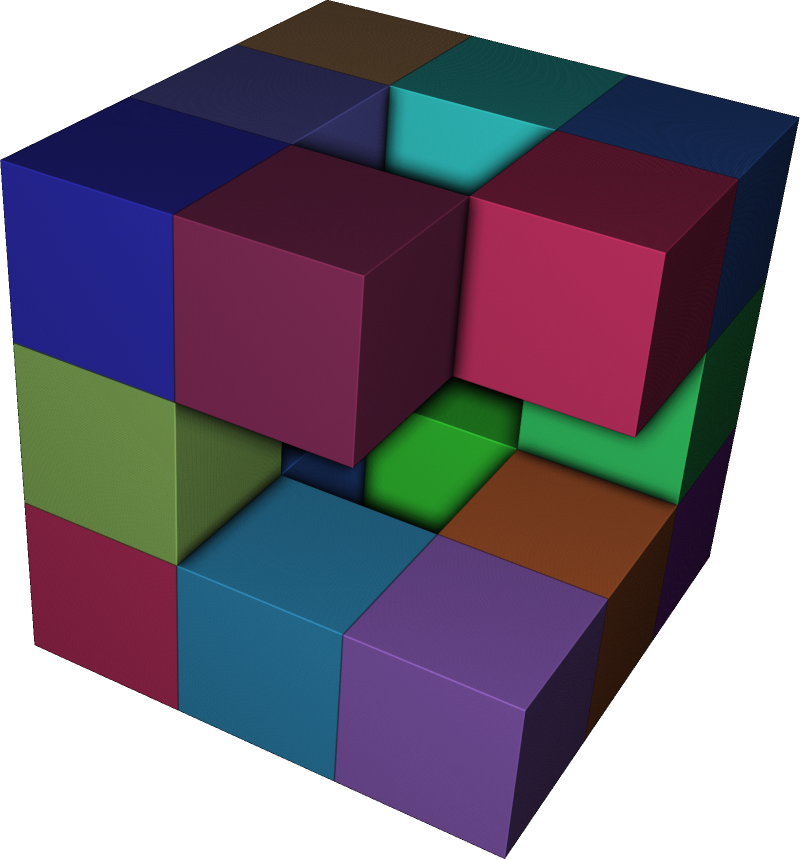
\includegraphics[width=0.4\textwidth]{FQD.png}
    \hfill
    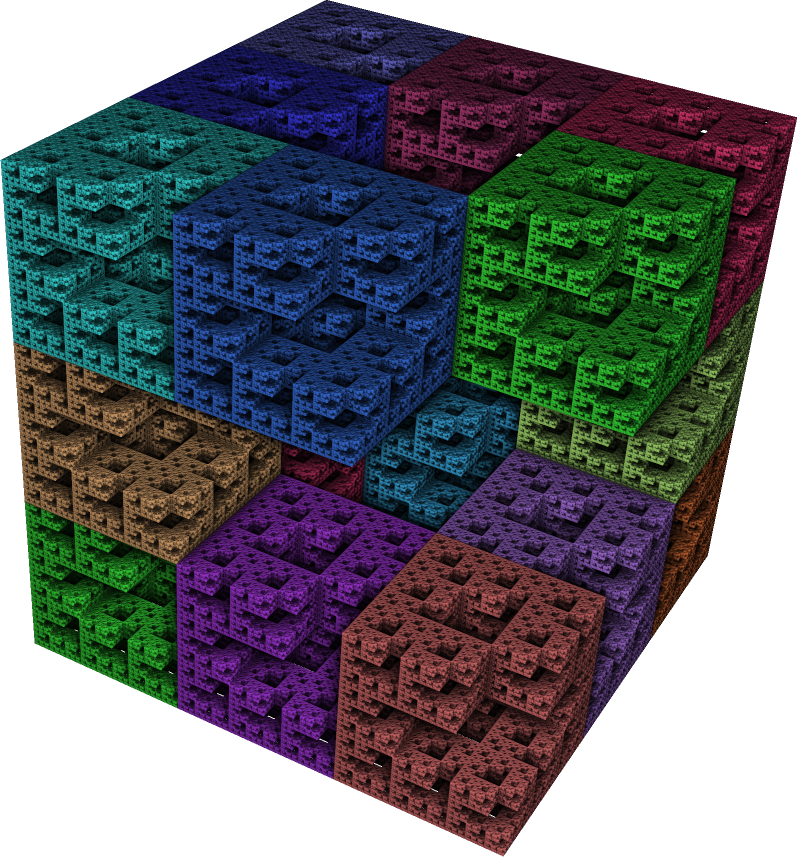
\includegraphics[width=0.4\textwidth]{FQK.png}
    \qquad
    \caption{Множество $D+P$ (слева) и фрактальный куб $nK=K+D$ (справа)}
    \label{fig:FQ}
\end{figure}

В случаях, когда $k=2$ и $k=3$, мы называем $K$ \emph{фрактальным квадратом} и \emph{фрактальным кубом} сответственно.

Уравнение \eqref{fqeq} можно использовать в его эквивалентной форме $nK=K+D$.
Само же множество $K$ содержится в единичном $k$-мерном кубе $P=[0,1]^k$, поскольку $P$ удовлетворяет уравнению $nP\NI P+D$.

Рассмотрим также эквивалентное определение фрактального $k$-куба $K$ порядка $n$ с множеством единиц $D$.
Возьмем единичный $k$-куб $P$ и разобьем его на $n^k$ равных $k$-кубов с ребром $1/n$.
Нижний ближайшая к нулю вершина каждого маленького $k$-куба $P_i$ имеет координату вида $\dfrac{d_i}{n}$, где $d_i\in\{0,1,\ldots,n-1\}^k$.
Из этого разбиения выберем те $k$-кубы $P_i$, для которых $d_i\in D$ (см. пример на рисуноке \ref{fig:FQ}).
Гомотетия, переводящая $P$ в $P_i$, имеет вид $S_i(x)=\dfrac{x+d_i}{n}$.
Тогда $K=\bigcup\limits_{d_i\in D}\frac{d_i+K}{n}$.

Уравнение \eqref{fqeq} определяет систему $\eS$ гомотетий $S_i(x)=\dfrac{x+d_i}{n}$, где $d_i\in D$, а оператор Хатчинсона $T_\eS$ системы $\eS$ определяется уравнением $T_\eS(A)=\dfrac{D+A}{n}=\bigcup\limits_{d_i\in D}\dfrac{d_i+A}{n}$.

\begin{definition}\label{refin}
Для любого $m\in \nn$, {\em $m$-е измельчение} системы $\eS$ --- это система $\eS^m=\{S_\bi, \bi=i_1i_2\ldots i_m\in I^m\}$, где $S_\bi(x)=\dfrac{x+d_\bi}{n^m}$ и $d_\bi=n^{m-1}d_{i_1}+n^{m-2}d_{i_2}+\ldots+d_{i_m}$. 
\end{definition}

Системе $\eS^m$ соответствует аттрактор $K$ как фрактальный $k$-куб порядка $n^m$ с множеством единиц $D^m=n^{m-1}D+n^{m-2}D+\ldots+D$ и копиями $\dfrac{K+d_\bi}{n^m}$.
Оператор Хатчинсона $T_\eS^m$ этой системы $\eS^m$ определяется уравнением $T_\eS^m(A)=\dfrac{D^m+A}{n^m}$.

Каждой бесконечной строке $\bi=i_1i_2\ldots\in I^\8$ соответствует единственная точка $x=\pi(\bi)$, где $\pi(\bi)=\sum\limits_{m=1}^\8 \dfrac{d_{i_m}}{n^m}$.

\begin{remark}% \label{rmk:fsd}
Далее, если не указано иное, говоря {\em <<фрактальный $k$-куб $K$>>}, мы будем иметь в виду {\em <<фрактальный $k$-куб $K$ порядка $n$ с множеством единиц $D$>>}. 
\end{remark}


\subsection{Грани $K_\al$ и пересечения граней $F_\al$ фрактального $k$-куба}

Единичный $k$-куб $P$ является фрактальным $k$-кубом порядка $n$ с множеством единиц $D=\{0,1,\ldots,n-1\}^k$, поскольку $P=\dfrac{P+\{0,1,\ldots,n-1\}^k}{n}.$
Значит, любой фрактальный $k$-куб $K$ содержится в единичном $k$-кубе $P$.

Если фрактальный $k$-куб $K$ является аттрактором системы $\eS$, то из включения $K\IN P$ следует $S_i(K)\IN S_i(P)$ для любого $S_i\in\eS$.
Более того, для любых $S_i, S_j\in\eS$ малые $k$-кубы $S_i(P)$ и $S_j(P)$ могут пересекаться друг с другом только по своим граням.
Прообразы этих граней в $S_i(P)$ и $S_j(P)$ относительно соответственных отображений $S_i$ и $S_j$ являются парой противоположных граней в $P$.
Введём обозначения для граней $k$-куба $P$ и пересечений этих граней с фрактальным $k$-кубом $K$.

Рассмотрим множество векторов $A=\{-1,0,1\}^k$.
Между множеством $A$ и множеством граней единичного $k$-куба $P=[0,1]^k$ существует взаимно-однозначное соответствие.

\begin{definition}\label{dfn:Pa}
Каждому вектору $\bma\in A=\{-1,0,1\}^k$ соответствует грань $P_\bma:=P\cap(P+\bma)$ единичного $k$-куба $P$.
\end{definition}

Симметрия противоположных граней $k$-куба $P$ выражается равенством 
$$P_\bma=P\cap(P+\bma)=((P-\bma)\cap P)+\bma=P_{-\bma}+\bma.$$

\begin{figure}[h!]
 \centering
 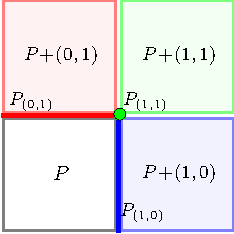
\includegraphics[width=0.45\textwidth]{faces_p.pdf}
 \hfill
 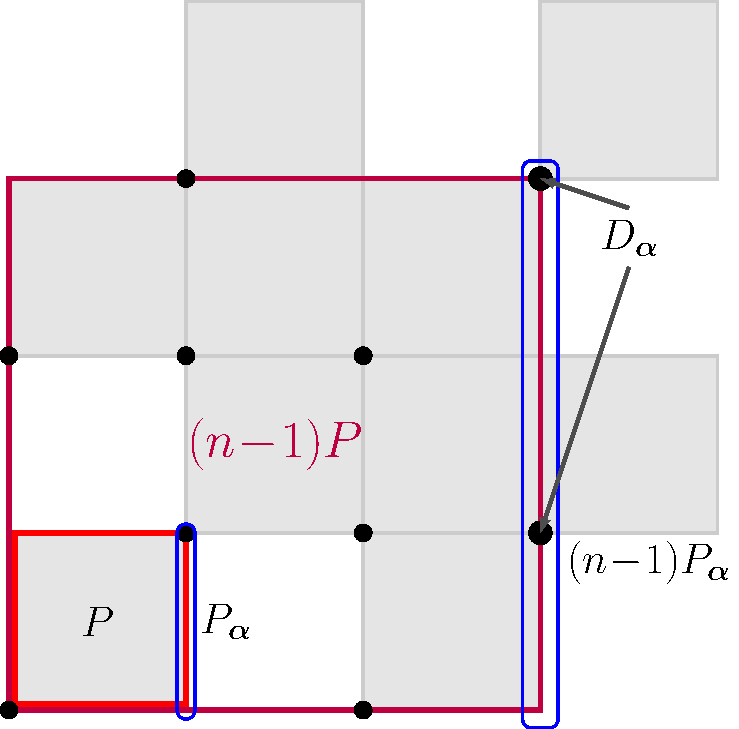
\includegraphics[width=0.45\textwidth]{faces_k.pdf}
 \caption{Множества $P_\bma$ и $D_\bma.$}
 \label{fig:faces}
\end{figure}

Введём отношение порядка $\sqsubseteq$ на $A$, равносильное отношению включения $\supseteq$ граней $k$-куба $P$:

\begin{definition}\label{Aorder}
Пусть $\bma=(\al_1,\al_2,\ldots,\al_k)$, $\bmb=(\be_1,\be_2,\ldots,\be_k)\in A$.
Будем говорить, что $\bma\sqsubseteq\bmb$, если из $\al_i\neq 0$ следует $\be_i=\al_i$.
Если при этом $\bma\neq\bmb$, то $\bma\sqsubset\bmb$.
\end{definition}

Очевидно, что $\bma\sqsubseteq\bmb$ тогда и только тогда, когда $P_\bma\supseteq P_\bmb$. 
Максимальными элементами из $A$ по отношению $\sqsubseteq$ являются векторы $(\pm 1,\ldots,\pm 1)$, которым соответствуют вершины $k$-куба $P$.
Минимальным элементом из $A$ по отношению $\sqsubseteq$ является $0$, которому соответствует единичный $k$-куб $P=P_{0}$.

\begin{definition}\label{def:K_alpha}
Гранью $K_\bma$ фрактального $k$-куба $K$ называется множество $K\cap P_\bma$.
\end{definition}

\begin{figure}[h!]
\centering
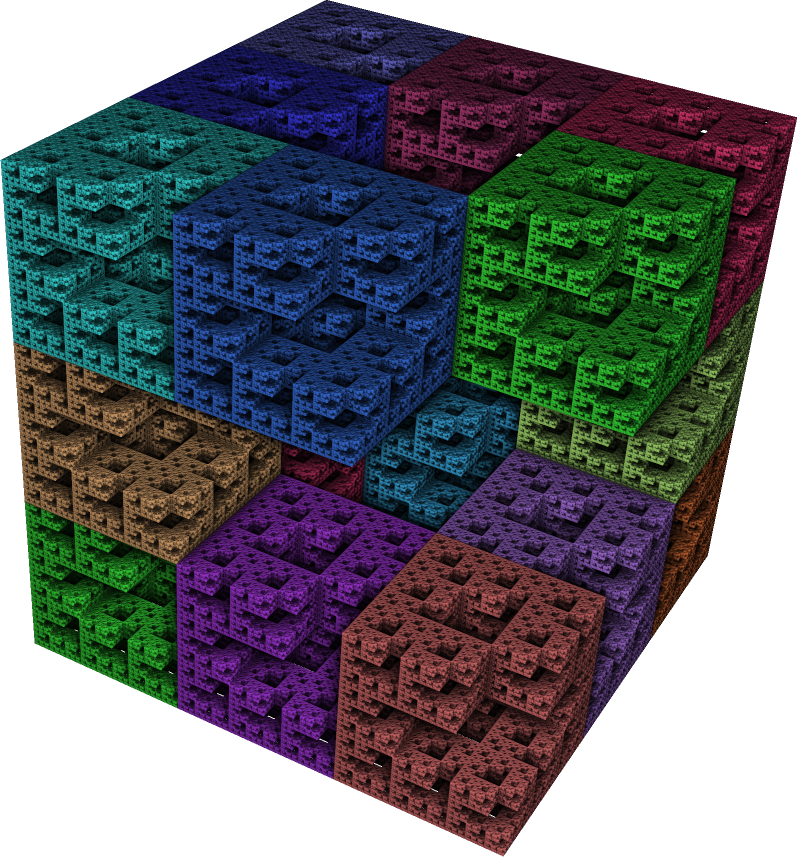
\includegraphics[width=0.45\textwidth]{images/presentation/qK.png}
 \hfill
 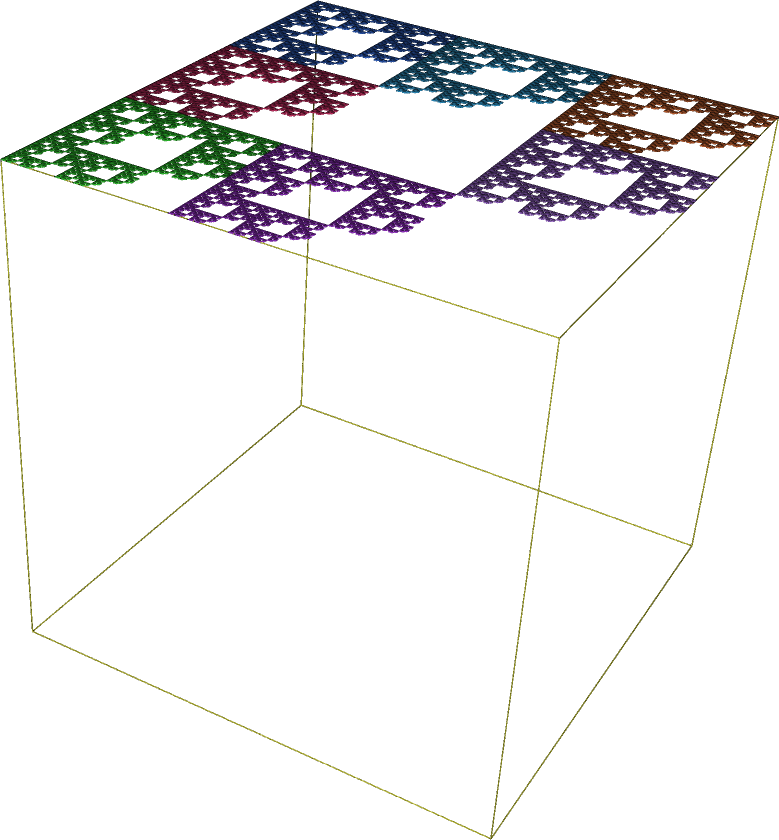
\includegraphics[width=0.45\textwidth]{images/presentation/qK_a.png}
  \caption{Фрактальный куб $K$ и его грань $K_\bma$}
 \label{fig:qK_a}
\end{figure}

\begin{proposition}\label{prop:Ka}
Грань $K_\bma$ фрактального $k$-куба $K$ удовлетворяет уравнению $n K_\bma=K_\bma+D_\bma$, где $D_\bma=D\cap(n-1)P_\bma$.
\end{proposition}

\begin{proof}
Заметим, что $n(K\cap P_\bma)=(K+D)\cap nP_\bma.$ 
Если $d\in D$ и \linebreak $d\notin(n-1)P_\bma$, то множество $(d+K)\cap nP_\bma$ пусто.
Поэтому мы будем рассматривать только те $d\in D$, для которых $d\in D\cap (n-1)P_\bma$.\\ 
Тогда $(d+K)\cap nP_\bma=d+K_\bma$, следовательно $n K_\bma={K_\bma+D_\bma}$.
\end{proof}

\begin{definition}\label{def:F_alpha}
Пусть даны фрактальные $k$-кубы $K^1$ и $K^2$.
Символом $F_\bma=F_\bma(K^1,K^2)$ обозначим пересечение $K^1_\bma\cap(K^2_{-\bma}+\bma)$ пары граней фрактальных $k$-кубов $K^1$ и $K^2$.
\end{definition}

Далее в тексте, если не указано иное, будем считать, что $K=K^1=K^2$.
Тогда $F_\bma$ есть пересечение $K_\bma\cap(K_{-\bma}+\bma)$ пары противоположных граней фрактального $k$-куба $K$.
В этом случае справедлива следующее предложение.

\begin{proposition}\label{fbma}
Пусть $K$ --- фрактальный $k$-куб.
\begin{itemize}[nolistsep]
\item[1.] Для любого $\bma\in A$ верно равенство $K\cap(K+\bma)=F_\bma=F_{-\bma}+\bma $;
\item[2.] Если $\bi,\bj \in I^k$, $\bi\neq \bj$ и $K_\bi\cap K_\bj\neq\0$, то $d_\bi-d_\bj=\bma$ для некоторого $\bma\in A$, и при этом 
$$K_\bi\cap K_\bj=\dfrac{d_\bi+F_\bma}{n^k}.$$
\end{itemize}
\end{proposition}

\begin{proof}
1. Поскольку $P\cap (P+\bma)=P_\bma=P_{-\bma}+\bma$, то мы имеем цепочку равенств 
$$K\cap(K+\bma)= K_\bma\cap (K_{-\bma}+\bma)=F_\bma=F_{-\bma}+\bma.$$

2. Заметим, что $S_\bi^{-1}(K_\bi\cap K_\bj)=K\cap S_\bi^{-1}(K_\bj)=K\cap (K+d_\bj-d_\bi)$. 
Так как $d_\bj-d_\bi\in\zz^k$, последнее пересечение может быть непусто только в том случае, если $d_\bj-d_\bi$ равно некоторому $\bma\in A$. 
В этом случае $K\cap(K+d_\bj-d_\bi)=F_\bma$.
Значит $K_\bi\cap K_\bj= S_\bi(F_\bma)= \dfrac{d_\bi+F_\bma}{n^k}$. 
\end{proof}

Из предложения \ref{fbma} следует, что для любого фрактального $k$-куба существует $\dfrac{3^k-1}{2}$ способов пересечения смежных копий одинакового размера (поскольку $F_\bma$ и $F_{-\bma}$ соответсвуют одному и тому же способу смежности копий). 
Любое из этих пересечений является образом множества из системы $\{F_\bma\ :\ \bma\in A\mmm\{0\}\}$ относительно некоторого отображения $S_\bi$. 

Для $\bma=(\al_1,\ldots,\al_k)\in A$ введём обозначение $|\bma|=\al_1+\ldots+\al_k$.
Пусть $K^1$ и $K^2$ --- фрактальные $k$-кубы порядка $n$ с множествоами единиц $D^1$ и $D^2$, и $F_{\bma}=K^1\cap(K^2+\bma)$.
Тогда при $|\bma|=k$ множество $F_{\bma}=\left(\frac{\al_1+1}{2},\ldots,\frac{\al_k+1}{2}\right)$, если $(n-1)\cdot\left(\frac{\al_1+1}{2},\ldots,\frac{\al_k+1}{2}\right)\in D^1$ и $(n-1)\cdot\left(\frac{-\al_1+1}{2},\ldots,\frac{-\al_k+1}{2}\right)\in D^2$, в противном случае $F_{\bma}=\0$. 
Иными словами, множества $F_{(\pm1,\ldots,\pm1)}$ соответствуют пересечениям противоположных вершин $k$-куба $P$, а потому являются одноточечными или пустыми.

Уравнения, задающие множества $F_\bma$, получаются из следующей теоремы.

\begin{theorem}\label{thm:falpha}
Пусть $K^1$ и $K^2$ --- фрактальные $k$-кубы порядка $n$ с множествоами единиц $D^1$ и $D^2$.
Для $\bma\in A\mmm\{0\}$ множество $F_\bma=K^1_{\bma}\cap(K^2_{-\bma}+\bma)$ удовлетворяет уравнению
\begin{equation}\label{sideint}
F_\bma=\bigcup\limits_{\bmb\sqsupseteq\bma} \dfrac{F_\bmb+G_{\bma\bmb}}{n}
\end{equation}
где $G_{\bma\bmb}=D^1_\bma\cap(D^2_{-\bma}+n\bma-\bmb)$.
\end{theorem}

Множество $G_{\bma\bma}=D_\bma\cap(D_{-\bma}+(n-1)\bma)$ мы для удобства обозначим как $G_{\bma}$.

\begin{proof}
Поскольку $P\cap (P+\bma)=P_\bma=P_{-\bma}+\bma$, то справедлива цепочка равенств
\begin{multline}\label{line}
nF_\bma=nK^1_\bma\cap (nK^2_{-\bma}+n\bma)=nK^1\cap(nK^2+n\bma)=\\
=(K^1+D^1)\cap(K^2+D^2+n\bma)=
\bigcup\limits_{d_1\in D^1,\ d_2\in D^2}(K^1+d_1)\cap (K^2+d_2+n\bma).
\end{multline}
Из соотношения $(K^1+d_1)\cap (K^2+d_2+n\bma)\neq\0$ следует, что $d_2-d_1+n\bma=\bmb$ для некоторого $\bmb\in A$.

Рассматривая $i$-ю координату в последнем равенстве, мы получаем
$$d_{2i}-d_{1i}+n\al_i=\be_i.$$ 
Из соотношений $\al_i,\be_i\in\{-1,0,1\}$ и $|d_{2i}-d_{1i}|\le n-1$ следует, что: \medskip
\begin{itemize}[nolistsep]
 \item[1.] если $\al_i=1$, то $\be_i>0$, а значит $\be_i=\al_i$ и $d_{2i}-d_{1i}=n-1$;
 \item[2.] если $\al_i=-1$ , то $\be_i<0$, поэтому $\be_i=\al_i$ и $d_{2i}-d_{1i}=1-n$;
 \item[3.] если $\al_i=0$ то $d_{2i}-d_{1i}=\be_i\in\{-1,0,1\}$.
\end{itemize} 
\medskip

%{\bf По Определению \ref{Aorder}, при $\bmb\sqsupseteq\bma$ существует три возможных варианта $\bmb$ если $0\in\{\al_1,\al_2\}$.}\\
%Если в $\bma$ одна из координат равна $0$, то есть $P_\bma$ --- ребро квадрата $P$, то существует три таких $\bmb$, что $\bmb\sqsupseteq\bma$
% Если $\bma$ --- индекс ребра, то существует три таких $\bmb$, что $\bmb\sqsupseteq\bma$.
Равенство $d_1=d_2+n\bma-\bmb$ показывает, что $d_1$ принадлежит множеству $D^1\cap(D^2+n\bma-\bmb)$, которое мы обозначим через $G_{\bma\bmb}$.
Каждое $d_1\in G_{\bma\bmb}$ задаёт единственное $d_2$ и для них справедливы равенства 
$$(K^1+d_1)\cap (K^2+d_2+n\bma)= (K^1\cap(K^2+\bmb))+d_1= F_\bmb+d_1,$$ 
из которых следует, что $nF_\bma= \bigcup\limits_{\bmb\sqsupseteq\bma} {F_\bmb+G_{\bma\bmb}}$.
\end{proof}

\begin{corollary}
Если $\bma\in\{(1,0),\ (-1,0),\ (0,1),\ (0,-1)\}$, то $F_\bma$ связно тогда и только тогда, когда оно является отрезком.
\end{corollary}

\begin{proof}
Если $F_\bma$ связно, то множества $K_{\bma}$ содержит неодноточечное связное подмножество, значит $\dim_H(K_{\bma})\geq1$.
В силу Предложения \ref{prop:Ka} множество $K_{\bma}$ имеет размерность $\dim_H(K_{\bma})=\log_n\#D_{\bma}$.
Поскольку $\#D_{\bma}\leq n$, неравенство $\dim_H(K_{\bma})\geq1$ возможно только если $\#D_{\bma}= n$.
Такому множеству единиц $D_{\bma}$ сответствует фрактальный квадрат $K_{\bma}$, совпадающий с ребром $P_{\bma}$.

Аналогично, $K_{-\bma}=P_{-\bma}$.
Из этого следует, что $F_\bma=K_{\bma}=P_{\bma}$.
\end{proof}


\subsection{Мощность пересечений копий фрактального квадрата}

Рассмотрим фрактальный квадрат $K=\dfrac{K+D}{n}$ и пару таких копий $\dfrac{K+d_1}{n}$ и $\dfrac{K+d_2}{n}$, что $d_2=d_1+\bma$, где $\bma\in A\mmm\{0\}$.
Назовём такую пару копий {\em копиями с $\bma$-соседством}.
Тогда $\dfrac{K+d_1}{n}\cap\dfrac{K+d_2}{n}=\dfrac{d_1+F_\bma}{n}$, значит мощность пересечения копий с $\bma$-соседством совпадает с мощностью множества $F_\bma$.
Уравнение \eqref{sideint} в Теореме \ref{thm:falpha} позволяет нам оценить мощность множества $F_\bma$.

\begin{theorem}\label{fin_int}
Пусть $K=\dfrac{K+D}{n}$ --- фрактальный квадрат. Рассмотрим $F_\bma, \bma\in A\mmm\{0\}$.
\begin{itemize}[nolistsep]
 \item[(i)] Если $\#G_{\bma\bma}> 1$, то множество $F_\bma$ несчётно.
 \item[(ii)] Если $\#G_{\bma\bma}=1$ и существует $\bmb\sqsupset\bma$ такое, что  $F_\bmb$ непусто и $\#G_{\bma\bmb}\geq1$, то $F_\bma$ бесконечное счётное.
 \item[(iii)] Множество $F_\bma$ конечно в следующих случаях:
 \begin{itemize}[nolistsep]
 \item[\textbf{(a)}] $\#G_{\bma\bma}=1$ и $\#F_\bmb\cdot\#G_{\bma\bmb}=0$ для каждого $\bmb\sqsupset\bma$;
 \item[\textbf{(b)}] $\#G_{\bma\bma}=0$ и существует $\bmb\sqsupset\bma$ такое, что $\#F_\bmb\cdot\#G_{\bma\bmb}\geq1$.
 \end{itemize}
\end{itemize} 
\end{theorem}

\begin{proof}
При $\bma\in A\mmm\{0\}$ множество $F_\bma$ удовлетворяет уравнению
$F_\bma=\bigcup\limits_{\bmb\sqsupseteq\bma} \dfrac{F_\bmb+G_{\bma\bmb}}{n}$, 
где $G_{\bma\bmb}=D_\bma\cap(D_{-\bma}+n\bma-\bmb)$.\\
Если $\bma\in\{(1,0),\ (-1,0),\ (0,1),\ (0,-1)\}$, то $\#\{\bmb:\bmb\sqsupset\bma\}=2$, при этом $\bmb\in\{(1,1),\ (-1,1),\ (1,-1),\ (-1,-1)\}$.\\
Если $\bma\in\{(1,1),\ (-1,1),\ (1,-1),\ (-1,-1)\}$, то $\#\{\bmb:\bmb\sqsupset\bma\}=0$.\\

Для $\bma\in\{(1,1),\ (-1,1),\ (1,-1),\ (-1,-1)\}$, то $\#G_{\bma\bmb}\leq1$ множество $F_\bma$ не более чем одноточечно.\\

Далее предполагаем, что $\bma\in\{(1,0), (-1,0), (0,1), (0,-1)\}$.\\

(i) Если $\#G_{\bma\bma}> 1$, то $F_\bma$ содержит в себе фрактальный квадрат с множеством единиц $G_{\bma\bma}$, который имеет мощность континуума.\\

(ii) Рассмотрим случай, когда $\#G_{\bma\bma}=1$ и существует $\bmb\sqsupset\bma$ такое, что  $F_\bmb$ непусто и $\#G_{\bma\bmb}\geq1$. 
Такое непустое $F_\bmb$ единственно, поскольку иначе $\#G_{\bma\bma}>1$.
Множество $\dfrac{F_\bmb+G_{\bma\bmb}}{n}$ конечно, поэтому $F_\bma=\bigcup\limits_{n=1}^\8 S_\bma^n$.\\

(iii.{\bf a}) Пусть $G_{\bma\bma}=\{d_i\}$ и $\#F_\bmb\cdot\#G_{\bma\bmb}=0$ для каждого $\bmb\sqsupset\bma$.
В этом случае из равенства $F_\bma=\dfrac{F_\bma+\{d_i\}}{n}$следует $F_\bma=\left\{\dfrac{d_i}{n-1}\right\}$.\\

(iii.{\bf b}) Наконец, рассмотрим случай, когда $G_{\bma\bma}=\0$ и существует $\bmb\sqsupset\bma$ такое, что $\#F_\bmb\cdot\#G_{\bma\bmb}\geq1$.
При $G_{\bma\bma}=\0$ может существовать не более одного $\bmb\sqsupset\bma$ такого, что $F_\bmb\neq\0$, в противном случае $\#G_{\bma\bma}\geq2$.
Так как $\#F_\bmb=1$, множество $F_\bma=\dfrac{F_\bmb+G_{\bma\bmb}}{n}$ конечно, а говоря точнее, $\#F_\bma=\#G_{\bma\bmb}$.
\end{proof}

Далее докажем, что фрактальный квадрат, являющийся дендритом, обладает свойством одноточечного пересечения.
Поэтому укажем условия, при которых $F_\bma$ одноточечно:

\begin{corollary}\label{onepoint} 
Множество $F_\bma$ одноточечно, если \\
\textbf{(a)} $\#G_{\bma\bma}=1$ и $\#F_\bmb\cdot\#G_{\bma\bmb}=0$ для каждого $\bmb\sqsupset\bma$; или\\
\textbf{(b)} $\#G_{\bma\bma}=0$ и существует $\bmb\sqsupset\bma$ такое, что $\#F_\bmb\cdot\#G_{\bma\bmb}=1$.
\hfill\qed
\end{corollary}
 
 
Следующая теорема устанавливает отношения между множествами $F_\bma$:

 
\begin{theorem}\label{IFC}
Семейство $\{F_\bma, \bma\in A_k\}$ пересечений $F_\bma =K_{1}\cap (K_{2}+\bma)$ удовлетворяет системе $\Sa$ уравнеий
 
\begin{equation}\label{perall}
F_\bma=\bigcup\limits_{\bmb\sqsupseteq{\bma}}T_{\bma\bmb}(F_\bmb),\qquad \bma\in A_k,
\end{equation}
 
где для каждого $\bmb\sqsupseteq\bma$, 
\begin{equation}\label{Gab}
T_{\bma\bmb}(F_\bmb)=\frac{1}{n}(F_\bmb+G_{\bma\bmb})\mbox{\quad  \text{и} \quad}
  G_{\bma\bmb}=D_1\cap(D_2+n\bma-\bmb)
\end{equation}
\end{theorem}

 

\begin{proof}
Представим $F_\bma$ как $K_1\cap (K_2+\bma)=\dfrac{1}{n}\bigl((K_1+D_1)\cap (K_2+D_2+n\bma)\bigr).$ \\

Пусть $d_1\in D_1$ и $d_2\in D_2$, тогда пересечение $(K_{1}+d_1)\cap (K_{2}+d_2+n\bma)$ непусто если $(P+d_1)\cap (P+d_2+n\bma)\neq\0$, что означает, что вектор $\bmb=d_2-d_1+n\bma$ лежит в множестве $A$. 
Поскольку для любого номера координаты $i=1,\ldots  ,k$ мы имеем $|(d_2-d_1)_i|\le n-1$, это возможно только если $\bmb\sqsupseteq \bma$.\\

Если $\bmb=\bma$, то $d_1=d_2+(n-1)\bma$, следовательно $d_1\in D_1\cap(D_2+(n-1)\bma)= G_\bma$.

Если $\bmb\sqsupset\bma$, то $(K_{1}+d_1)\cap (K_{2}+d_2+n\bma)=(K_1\cap (K_2+\bmb))+d_1$, и $d_1\in D_1\cap(D_2+n\bma-\bmb)$. Множество $D_1\cap(D_2+n\bma-\bmb)$ мы обозначим как  $G_{\bma\bmb}$. 

Заметим, что  $G_{\bma\bma}=D_1\cap(D_2+n\bma-\bma)$, а значит $G_{\bma\bma}=G_{\bma}$.

В результате мы получаем  $F_\bma=\frac{1}{n}\bigcup\limits_{\bmb\sqsupseteq{\bma}}(F_\bmb+G_{\bma\bmb})=
\frac{1}{n}(F_\bma+G_\bma)\cup\bigcup\limits_{\bmb\sqsupset{\bma}}\frac{1}{n}(F_\bmb+G_{\bma\bmb})$.
\end{proof}\bigskip

Отношения между множествами $F_\bma$, установленные в Теореме \ref{IFC} приводят к {\em структурному графу $\Ga_\Sa$} системы $\Sa$, определенной в \eqref{perall}. 
С помощью этой систему и графа можно найти важные свойства множеств $F_\bma$.

\begin{definition}
Структурный граф $\Ga_\Sa$ является ориентированным графом, в котором все вершины являются непустыми множествами $F_\bma$ и для каждого $\bma\sqsubseteq\bmb$ существует ребро $(F_\bma,F_\bmb)$, направленное из $F_\bma$ в $F_\bmb$ и соответствует оператору $T_{\bma\bmb}$, если этот оператор невырожденный.
\end{definition}

В общем случае граф $\Ga_\Sa$ будет содержать $3^k$ вершин и $5^k$ ребер, и $3^k$ из этих ребер являются циклами от $F_\bma$ к самому себе.
Мы помечаем каждое ребро символом $G_{\bma\bmb}$.\\

Тем не менее, некоторые вершины и ребра в графе $\Ga_\Sa$ могут исчезнуть.
Это происходит для тех $F_\bma$, которые пусты, и для тех ребер $(F_\bma,F_\bmb)$, для которых $T_{\bma\bmb}(F_\bmb)=\0$, то есть 
\begin{equation}\label{Tempty}
T_{\bma\bmb}(F_\bmb)=\0\mbox{\quad   \text{если}  \quad  }G_{\bma\bmb}=\0\mbox{ \quad   \text{или} \quad   }F_\bmb=\0.
\end{equation} 

Множество $F_\bma$ пусто, если $G_\bma=\0$ и для любого $\bmb\sqsupset\bma$ множество $F_\bmb+G_{\bma\bmb}=\0$. 
Применяя \eqref{Tempty} ко всем $\bmb\sqsupset\bma$, мы выводим следующее условие пустоты для $F_\bma$:

\begin{lemma}
Множество $F_\bma=\0$ тогда и только тогда, когда для любого $\bmb\sqsupseteq\bma$ и для любой конечной последовательности\\ $\bma=\bma_0\sqsubseteq\bma_1\sqsubseteq\ldots \bma_{p-1}\sqsubseteq\bma_p=\bmb$ произведение 
$\#G_{\bma_0\bma_1}\#G_{\bma_1\bma_2}\ldots  \#G_{\bma_{p-1}\bma_p}\#G_{\bmb}$ равно нулю. 
\qed
\end{lemma}


По этим причинам, из-за сокращения всех пустых вершин и ребер, структурный граф $\Ga$ для системы $\Sa$, определенный в теореме \ref{IFC}, имеет множество вершин $V_\Sa=\{F_\bma: \bma\in A, F_\bma\neq\0\}$ и множество ребер
$E_\Sa=\{(F_\bma, F_\bmb): \bma\sqsubseteq\bmb, G_{\bma\bmb}\neq\0, F_\bmb\neq\0\}$. 

Вообще такой граф $\Ga_\Sa$ может быть и несвязен.

\begin{definition}
Мы говорим, что пара вершин $F_\bma, F_\bmb, \bma\sqsubset\bmb$ {\em соединена направленным путем} в графе $\Ga_\Sa$, если существует конечная последовательность  $\bma=\bma_0\sqsubset\bma_1\sqsubset\ldots \bma_{p-1}\sqsubset\bma_p=\bmb$ такая, что для любых  $j=0,\ldots  ,p$ множества $F_{\bma_j}\neq\0$  и множества $G_{\bma_{j-1}\bma_j}\neq\0$ для $j=1,\ldots  ,p$.   
\end{definition}

Мы пишем $\bmb\succ\bma$, если в $\Ga$ есть направленный путь от $F_\bma$ до $F_\bmb$.

Если $\bmb\succcurlyeq\bma$ или $\bma\succcurlyeq\bmb$, то мы говорим, что $\bma$ и $\bmb$ являются $\Ga${\em-сравнимы}.

Мы обозначим через $\Ga_\bma$ подграф в $\Ga$, все вершины которого являются $F_\bmb$ такими, что $\bmb\succcurlyeq\bma$. 
Мы говорим, что $\bmb$ является {\em максимальным} для $\Ga_\bma$, если $\Ga_\bmb$ является единственной вершиной $F_\bmb$.
Мы говорим, что $\bmb$ является {\em минимальным} для $\Ga_\Sa$, если нет $\bma$ такого, что $\bma\prec\bmb$.

Стоит отметить, что, согласно предложению \ref{falfa}, граф $\Ga_\bma$ показывает множество всех уравнений, которые полностью определяют каждое из множеств $F_\bmb$, для которых $\bmb\succcurlyeq\bma$.\\

Каждый оператор $T_{\bma\bmb}$, соответствующий некоторому ребру в графе $\Ga_\Sa$, является непустым конечным объединением гомотетий, поэтому он сохраняет размерность, т.е. для любого подмножества $X\IN F_\bmb$, $\dim_H(T_{\bma\bmb}(X))=\dim_H(X)$.\\


\begin{example} 
[Пересечение двух фрактальных квадратов, состоящее из $24$ точек, и его стркутурный граф $\Ga_\Sa$.]

Рассмотрим пересечение фрактальных квадратов $K_1$ и $K_2$ порядка $6$ с множествами единиц $D_1$ и $D_2$.
На рисунке слева ниже мы представляем множества единиц множеством красных клеток $T_1(P)=\dfrac{D_1+P}{6}$ и синих клеток $T_2(P)=\dfrac{D_2+P}{6}$ .
Справа видны фрактальные квадраты $K_1$ и $K_2$. \\

Большинство из множеств $G_\bma$, а именно, \\
$G_0,G_{(1,0)},G_{(-1,0)},G_{(0,1)},G_{(0,-1)},G_{(1,1)},G_{(1,-1)},G_{(-1,1)}$ являются пустыми, и только $G_{(-1,-1)}=(0,0)$. Следовательно, 
$F_{(1,1)}=F_{(1,-1)}=F_{(-1,1)}=\0$ и $F_{(-1,-1)}=\{(0,0)\}$.\\


\begin{figure}[H]
    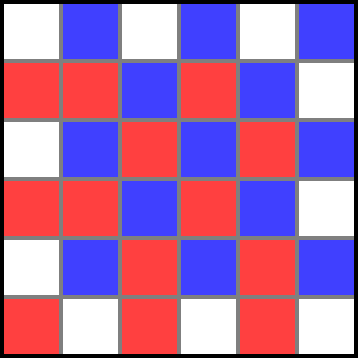
\includegraphics[width=0.45\textwidth]{FSI_6x6_DS.pdf}
    \hfill
    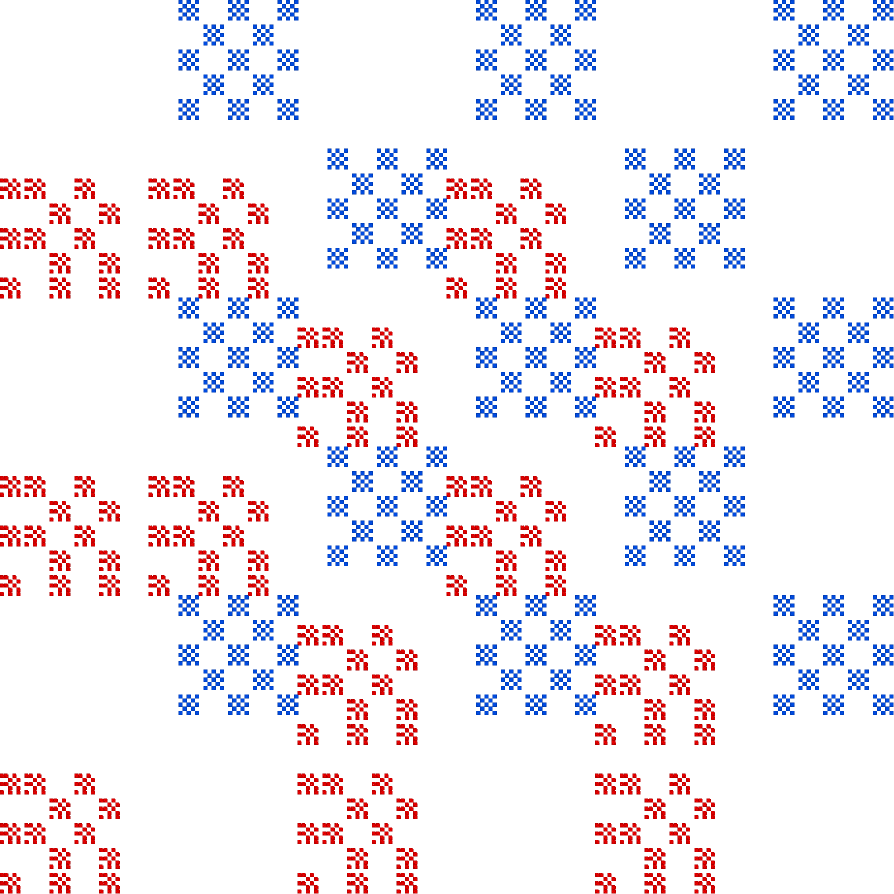
\includegraphics[width=0.45\textwidth]{FSI_6x6_K.png}
    \caption{Диаграмма множеств единиц для $D_1$ и $D_2$ (слева) и фрактальные квадраты $K_1$ и $K_2$ (справа).}
    % \label{fig:my_label}
\end{figure}


Множество $F_{(1,0)}$ пусто, поскольку $G_{(1,0)},F_{(1,1)}$ и $F_{(1,-1)}$ пусты. 
По той же причине $F_{(0,1)}=\0$. \\

Множества $G_{(-1,0)(-1,-1)}=\{(0,2),(0,4)\}$ и \\
$G_{0(-1,0)}=\{(1,2),(1,4),(2,3),(3,2),(3,4),(4,3)\}$.
Множества $G_{(0,-1)(-1,-1)}$ и $G_{0(0,-1)}$ получены их предыдущих двух.\\

Таким образом, после удаления пустых вершин и ребер
граф $\Ga_\Sa$ содержит четыре вершины  $F_0,F_{(-1,0)},F_{(0,-1)},F_{(-1,-1)}$ и четыре ребра, которым соответствуют $G_{(-1,0)(-1,-1)}, G_{(0,-1)(-1,-1)},G_{0(-1,0)}$ и $G_{0(0,-1)}$.

Вычисление с использованием формулы \eqref{perall} показывает, что
$\#F_{(-1,0)}=\#F_{(0,-1)}=2$ и $\#F_0=2 \#G_{0(-1,0)}+2\#G_{0(0,-1)}=24.$


\begin{figure}[H]
    \centering
    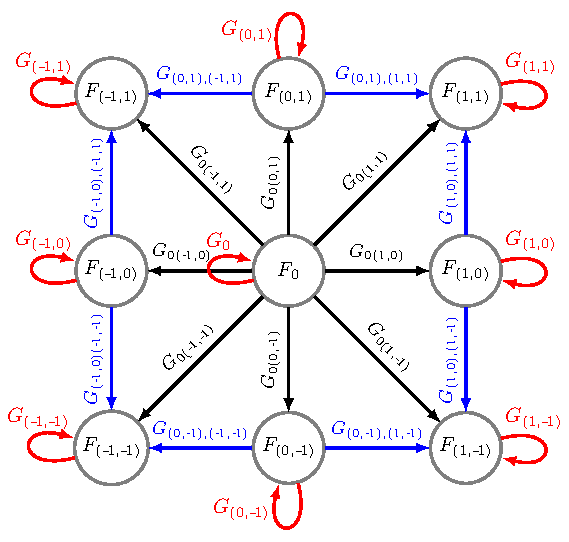
\includegraphics[width=.5\textwidth]{structure_grapg_full.pdf}
    \hfill
    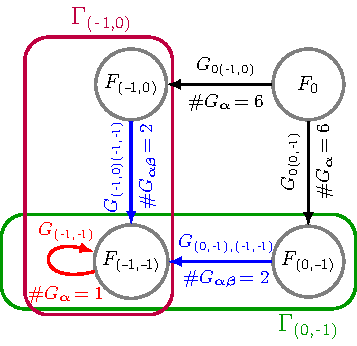
\includegraphics[width=.45\textwidth]{FSI_6x6_SG.pdf}
    \caption{Структурный граф $\Ga_\Sa$ в общем случае для пересечения двух фрактальных квадратов (слева) и сокращённый граф $\Ga_\Sa$ для Примера 1 (справа). На рисунке справа выделены подграфы $\Ga_{(-1,0)}$ и $\Ga_{(0,-1)}$. }
\end{figure} 
\end{example} 


\subsection{Мощность множества $F_\al$.}

\begin{theorem}\qquad
\begin{enumerate}[nolistsep]
\item Множество $F_\bma$ является одноточечным, если $\Gamma_\bma$ представляет собой цепочку $\bma=\bma_1\prec\ldots\prec\bma_p$, в которой для всех $j\le p-1$, $\# G_{\bma_j\bma_{j+1}}=1$, $G_{\bma_j}=\0$ и $\#G_{\bma_p}=1$;
\item Множество $F_\bma$ конечно, если для всех максимальных вершин $\bmb$ в $\Gamma_\bma$, верно $\#G_\bmb=1$ и $G_{\bmb}=\0$ для всех остальных вершин в $\Gamma_\bma$.
В этом случае $\#F_\bma$ равно сумме всех композиций $\prod \limits_{j=1}^{p-1}\# G_{\bma_j\bma_{j+1}}$, взятых по всем цепочкам $\bma=\bma_1\prec\ldots\prec\bma_p=\bmb$, где $\bmb$ является максимальным в $\Gamma_\bma$;
\item Множество $F_\bma$ счетно, если $\#G_\bmb\le 1$ для всех вершин $\bmb$ в $\Gamma_\bma$;
\item Множество $F_\bma$ несчетно, если в $\Gamma_\bma$ существует такая вершина $\bmb$, что $\#G_\bmb> 1$.
\end{enumerate}
\end{theorem}

\begin{corollary}
Фрактальный куб $K$ обладает свойством одноточечного пересечения, если структурный граф $\Gamma(\Sa)$ представляет собой объединение цепочек $0\prec\bma_{i1}\prec\ldots\prec\bma_{ip_i}$, для которых все $\bma_{ij}$ различны и таковы, что для всех $i$ верно $\#G_{\bma_{ip_i}}=1$ и для всех $i,j$ таких, что $j\le p_i-1$, верно $\# G_{\bma_{ij}\bma_{i,j+1}}=1$ и $G_{\bma_{ij}}=\0$.

Фрактальный куб $K$ обладает свойством конечного пересечения, если для всех максимальных $\bma$ в графе $\Ga (\Sa)$, $\#G_\bma=1$ и для всех остальных $\bma\neq 0$, $\#G_\bma=0$.
\end{corollary}

\begin{example}[Фрактальный куб с одноточечным пересечением]
Возьмем фрактальный куб $K=\dfrac{K+D}{4}$ с множеством единиц 
\begin{equation*}
\begin{split}
D=\{
    &(0,0,0), (1,1,1), (2,2,2), (3,3,3), (2,1,1), (1,2,1), (1,1,2), (1,2,2),\\ 
    &(2,2,1), (2,1,2), (0,0,2), (0,2,1), (3,3,1), (3,1,1), (2,0,0), (1,2,0),\\ 
    &(1,3,3), (1,1,3)\}     
\end{split}
\end{equation*}
 
\begin{figure}[H]
    \centering
    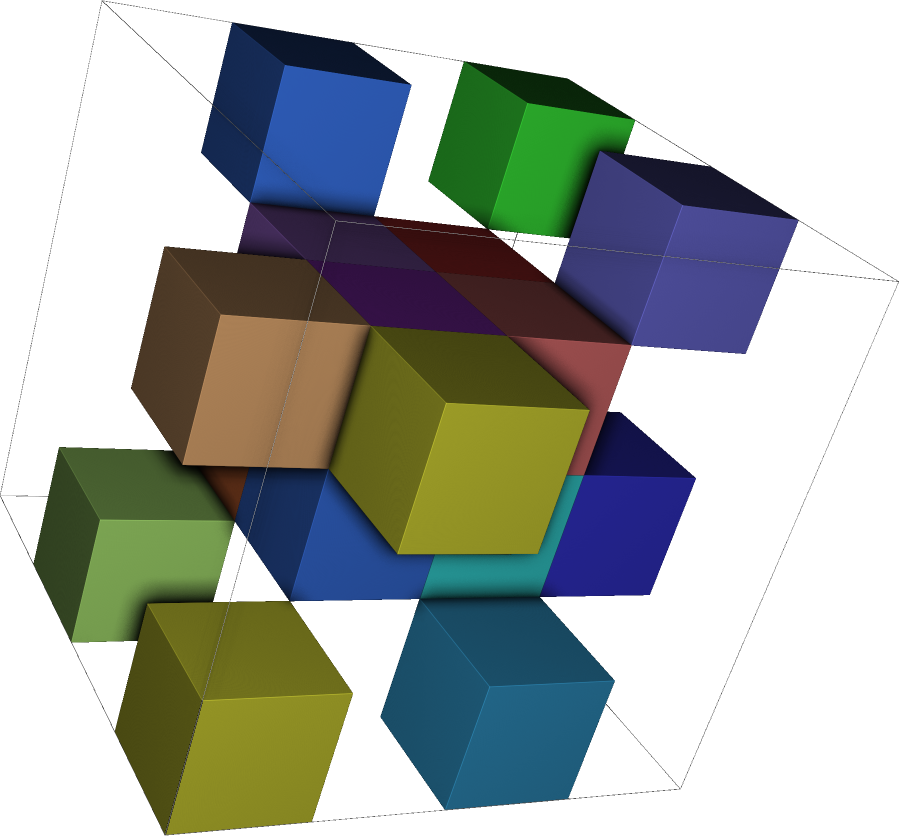
\includegraphics[width=0.45\textwidth]{fqP1a.png}
    \hfill
    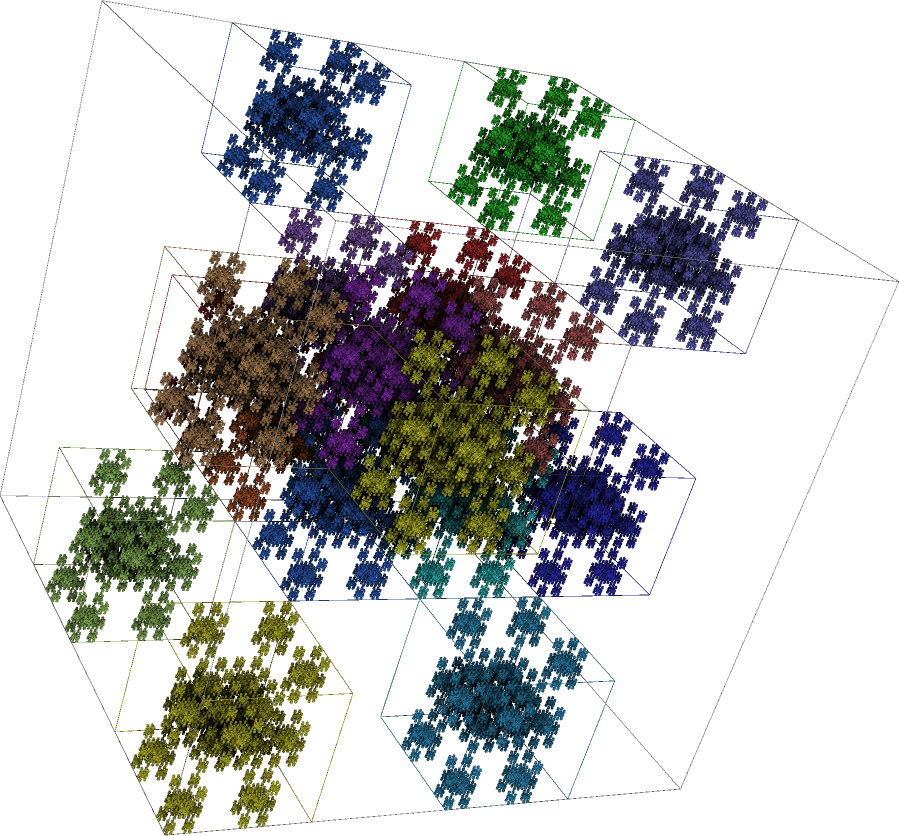
\includegraphics[width=0.45\textwidth]{fqK1a.png}
    \caption{Фрактальный куб с одноточечным пересечением}
    \label{fig:fq}
\end{figure}

\begin{figure}[H]
    \centering
    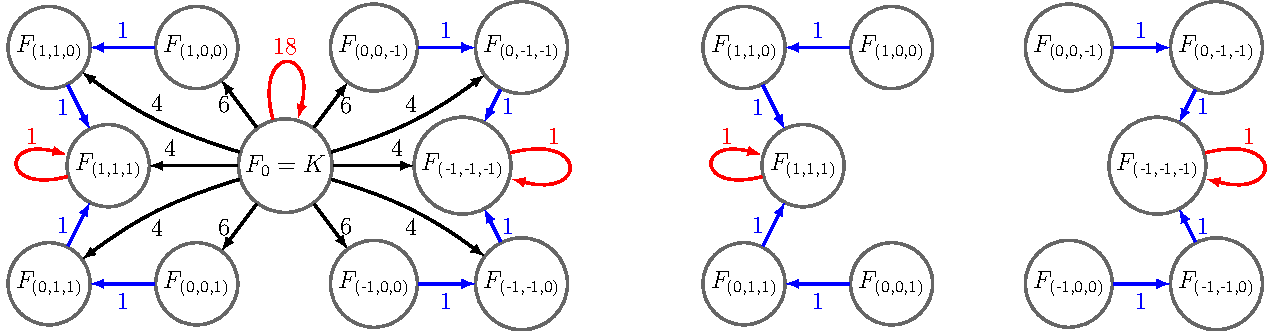
\includegraphics[width=\textwidth]{SG_for_FQ.pdf}
    \caption{Структурный граф}
    \label{fig:fq_sg}
\end{figure}
\end{example}

\begin{figure}[H]
    \centering
    \hfill
    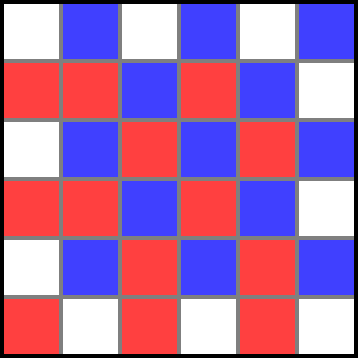
\includegraphics[width=0.45\textwidth]{FSI_6x6_DS.pdf}
    \hfill
    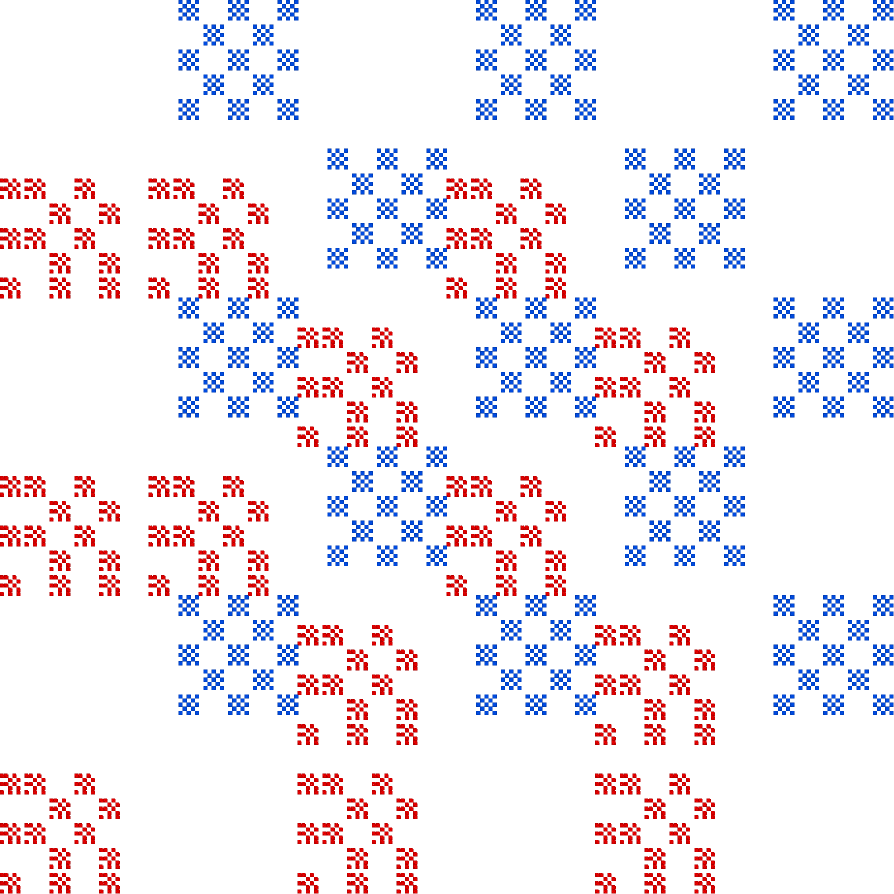
\includegraphics[width=0.45\textwidth]{FSI_6x6_K.png}
    \hfill
    \caption{Пересечение фрактальных квадратов по 24 точкам}
    \label{fig:FSI_6x6}
\end{figure}

\begin{example}[Пересечение по 24 точкам]
\label{ex:FSI_6x6}
На Рисунке \ref{fig:FSI_6x6} представлено пересечение двух фрактальных квадратов $K_1$ и $K_2$ порядка $6$ (синее и красное множество), а на Рисунке \ref{fig:FSI_SG} слева показан структурный граф $\Gamma_{\Sigma(K_1,K_2)}$ этого пересечения.
По этому графу легко понять, что пересечение $F_0$ конечно, причем $\#F_0=24.$
\end{example}



\section{Свойсво одноточечного пересечения и условие того, что фрактальный куб является дендритом}



\subsection{Свойство одноточечного пересечения и критерий дендритности}

Рассмотрим фрактальные $k$-кубы с одноточечным пересечением и проверим, является ли рассматриваемое множество дендритом.
\begin{definition}\label{fipss}\cite{FIP}
Система множеств с одноточечным пересечением (было в главе 1)  
\end{definition}

\begin{definition}\label{fipcs}
Система сжимающих подобий со свойством одноточечного пересечения.(было в главе 1)
\end{definition}

\subsection{Алгоритм проверки фрактального куба на свойство дендритности}

Пусть $K$ --- фрактальный $k$-куб.
Чтобы проверить $K$ на наличие дендритности, нужно выполнить следующие шаги:

 \begin{enumerate}

    \item Найдём все множества $G_\bma, G_{\bma\bmb}$ для системы $\Sigma=\Sigma(K,K)$ и запишем систему $\Sa$.
    Согласно Определению \ref{strg} и Лемме \ref{red}, исключим все исчезающие вершины и ребра и построим граф $\Ga_\Sa$.
   
    \item Используя Следствие \ref{SIPQ}, проверим выполнение свойства одноточечного пересечения для $K$.
    Если это не удается, то $K$ не является дендритом.
    
    \item Построим двудольный граф пересечений для фрактального куба $K$, соединив рёбрами пересекающиеся копии с точкой пересечения этих копий. 
    Нужно учесть случай с кратными точками, упомянутыми в следствии \ref{mpoint}.
    Теперь если получившийся двудольный граф пересечений будет деревом, то $K$ --- дендрит.
    
\end{enumerate}